%% ------------------------------------------------------------------------- %%
\chapter{Fundamentação Teórica}
\label{cap:conceitos}

{\color{red} Fazer uma breve introdução aqui.}

%% ------------------------------------------------------------------------- %%
\section{Modelos de Cores}\index{cores!modelos de}
\label{sec:fundamentos}

O uso de imagens coloridas em visão computacional ou no processamento de imagens pode ser motivado por dois fatores principais. O primeiro diz respeito a característica poderosa da cor de funcionar como um descritor que, frequentemente, simplifica a identificação e extração de um objeto em uma cena. O segundo está relacionado com a capacidade dos seres humanos de discernir milhares de tonalidades e intensidades, se comparado com apenas algumas dúzias de níveis de cinza \citep{gonzalez:02}.

A percepção visual da cor pelo olho humano não deve variar conforme a distribuição espectral da luz natural incidente sobre um objeto. Em outras palavras, a aparência de cor dos objetos permanece estável sob condições de iluminação diferentes. Esse fenômeno é conhecido como constância de cor \citep{gevers:12}.

Como exemplo, o gramado de um estádio de futebol permanece verde durante todo o dia, inclusive ao entardecer quando, de um ponto de vista físico, a luz solar
tem um aspecto mais avermelhado.

A percepção humana das cores se dá pela ativação de células nervosas que enviam
mensagens ao cérebro sobre brilho (\textit{brightness}), matiz (\textit{hue}) e 
saturação (\textit{saturation}) que, geralmente, são as características usadas
para distinguir uma cor de outra \citep{gonzalez:02}.

O brilho dá a noção de intensidade cromática. Matiz representa a cor dominante
percebida por um observador. Já a saturação refere-se à pureza relativa ou quantidade de luz branca aplicada ao matiz. Combinados, matiz e saturação são conhecidos como cromaticidade e, portanto, uma cor deve ser caracterizada por seu brilho e cromaticidade \citep{gonzalez:02}.

As cores podem ser especificadas por modelos matemáticos em tuplas de números em um sistema de coordenadas e um subespaço dentro desse sistema onde cada cor
é representada por um único ponto. Tais modelos são conhecidos como modelo de cores \citep{gonzalez:02}.

Esses modelos podem ser classificados como de dois tipos: os modelos aditivos em que as intensidades das cores primárias são adicionadas para produzir outras cores e subtrativos, onde as cores são geradas subtraindo-se o comprimento da onda dominante da luz branca.

As seções seguintes descrevem brevemente alguns dos principais modelos de cores, bem como seus variantes e principais áreas de aplicação.

%% ------------------------------------------------------------------------- %%
\subsection{Modelo de Munsell}\index{cores!modelo de Munsell}
\label{sec:modelo_cores_munsell}

Pioneiro na tentativa de organizar a percepção de cor em um espaço de cores, Albert H. Munsell conseguiu aliar a arte e a ciência das cores em uma única teoria \citep{konstantinos:00}.

O princípio da igualdade de espaçamento entre os componentes do modelo é a ideia principal do modelo de cores de Munsell \citep{konstantinos:00}. Esses componentes são matiz (\textit{hue}), luminosidade (\textit{value}) e saturação (\textit{chroma}).

O modelo é representado por uma forma cilíndrica e pode ser visto na figura~\ref{fig:munsell-system}. O matiz está disposto no eixo circular que consiste de
cinco cores de base e cinco secundárias, a saturação no eixo radial e a luminosidade no eixo vertical em uma escala variando de 0 a 10.

\begin{figure}[!h]
  \centering
  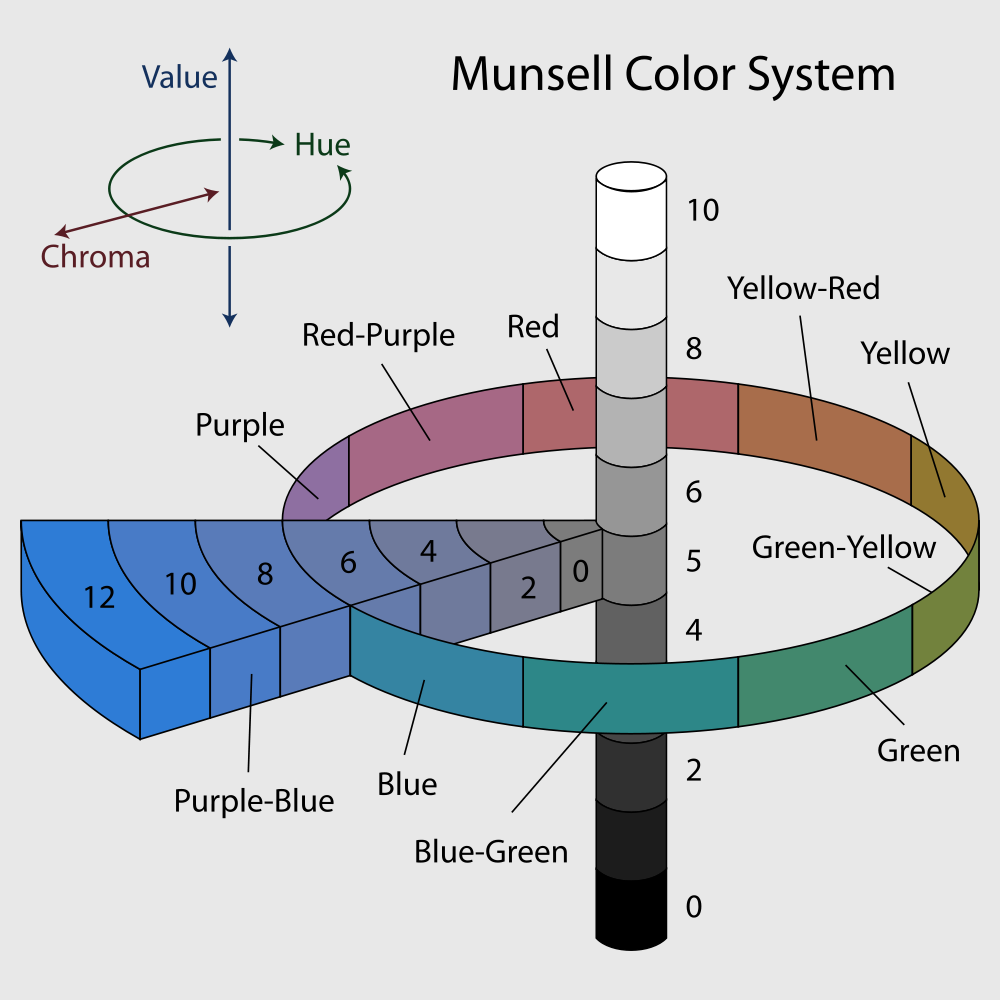
\includegraphics[width=.55\textwidth]{munsell-system}
  % fonte https://commons.wikimedia.org/wiki/File:Munsell-system.svg
  \caption{Modelo de cores de Munsell.}
  \label{fig:munsell-system} 
\end{figure}

%% ------------------------------------------------------------------------- %%
\subsection{Modelo CIE}\index{cores!modelo CIE}
\label{sec:modelo_cores_cie}

Em 1931, o CIE estabeleceu o primeiro modelo matemático de especificação numérica da cor, cujo objetivo era analisar a relação entre os aspectos físicos das cores no espectro eletromagnético e sua percepção pelo sistema visual humano para determinar como uma pessoa comum percebe a cor. Uma revisão desta especificação foi publicada em 1964 \citep{gonzalez:02}.

O experimento que originou o padrão consistia em detectar as cores percebidas por um observador a partir de uma mistura de três cores primárias X, Y e Z chamadas de valores tristímulus. Estas coordenadas deram origem ao espaço de cores \textbf{CIE XYZ} que engloba todas as cores que podem ser percebidas por um ser humano comum e, por esta razão, é considerado uma representação independente de dispositivo \citep{konstantinos:00}.

O sistema proposto pelo CIE XYZ para descrição de uma cor é baseado em um componente de luminância Y e outros dois componentes adicionais X e Z que dão a informação de cromaticidade. Esse sistema é formado por cores imaginárias que podem ser expressas como combinações das medidas normalizadas abaixo:


\begin{equation}
  x = \frac{X}{X + Y + Z}
\end{equation}

\begin{equation}
  y = \frac{Y}{X + Y + Z}
\end{equation}

\begin{equation}
  z = \frac{Z}{X + Y + Z}
\end{equation}

com $x + y+ z = 1$.

As combinações de valores negativos e outros problemas relacionados à seleção de um conjunto de primárias reais são eliminados.  As coordenadas de cromaticidade $x$ e $y$ permitem representar todas as cores num plano bidimensional, conhecido como diagrama de cromaticidade, que pode ser visto na figura~\ref{fig:cie-cromaticity-diagram}.

\begin{figure}[!h]
  \centering
  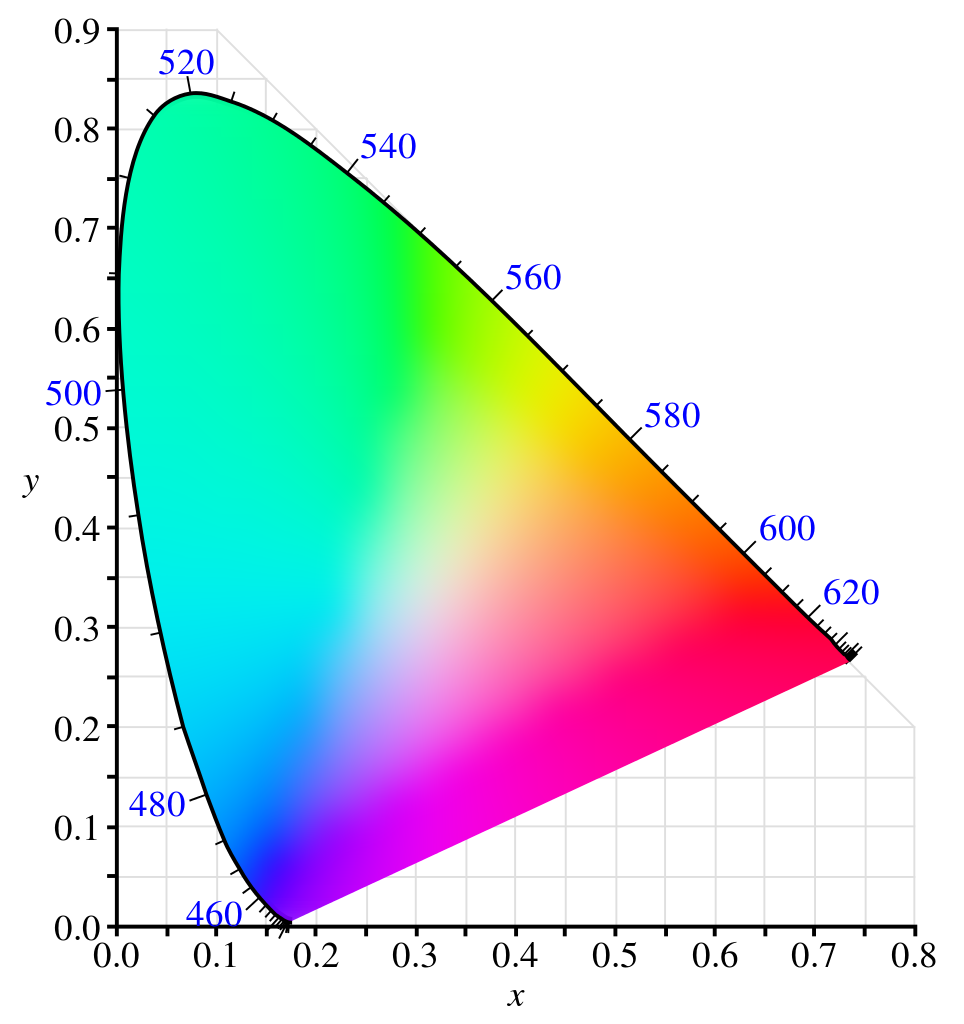
\includegraphics[width=.5\textwidth]{cie-cromaticity-diagram}
  % fonte https://en.wikipedia.org/wiki/File:CIE1931xy_blank.svg
  \caption{Diagrama de cromaticidade CIE 1931.}
  \label{fig:cie-cromaticity-diagram} 
\end{figure}

Os pontos que representam as cores puras no espectro eletromagnético são rotulados de acordo com os seus comprimentos de onda e estão localizados ao longo da curva que vai da extremidade direita do eixo $x$ correspondente à cor vermelha até a extremidade esquerda do mesmo eixo correspondente à cor violeta, formando um polígono parecido com uma ferradura. Os pontos internos correspondem a todas as combinações possíveis de cores visíveis. As coordenadas $(x = 1/3, y = 1/3)$ correspondem à localização da luz branca, também conhecida como ponto branco, e servem de referência no processo de captura de imagem, codificação ou reprodução.

O CIE também derivou e padronizou outros dois modelos de cores a partir da especificação do CIE XYZ e, da mesma maneira, são independente de dispositivo. Ambos são perceptualmente uniformes, ou seja, distâncias perceptuais iguais separam todas as cores \citep{vezhnevets:03}. Como exemplo, a escala de cinzas do espaço deve permitir uma transição suave entre o preto e o branco.

O primeiro deles foi concebido para reduzir o problema de não uniformidade perceptual. Alguns diagramas de Escala Uniforme de Cromaticidade (UCS) foram propostos com base em equações matemáticas para transformar os valores XYZ ou as coordenadas $x, y$ em um novo conjunto de valores $(u, v)$, o que deu origem ao diagrama de cromaticidade 1960 CIE $uv$ \citep{gevers:12}.

Ainda com resultados insatisfatórios, o CIE fez uma nova mudança multiplicando o componente $v$ por um fator 1,5. Além disso, a escala de luminosidade dada pelo componente Y foi substituída por $L^* = [0, 100]$ para melhor representar as diferenças na luminosidade que são equivalentes. Esta revisão originou o modelo de cores \textbf{CIE 1976 $L^*u^*v^*$}, comumente conhecido pela sigla CIELUV \citep{gevers:12}.

Em 1976 o CIE adotou um novo modelo de cores, baseado no modelo $L, a, b$, proposto por Richard Hunter em 1948, que melhor representava o espaçamento uniforme das cores. Denominado \textbf{1976 CIE $L^*a^*b^*$} e conhecido pela sigla CIELAB, é um espaço baseado em cores oponentes \footnote{Teoria iniciada por volta do ano de 1500 quando Leonardo da Vinci concluiu que as cores são produzidas pela mistura de amarelo e azul, verde e vermelho, e branco e preto. Em 1950 houve a confirmação desta teoria quando sinais de cores oponentes foram detectados na conexão óptica entre a retina e o cérebro \citep{gevers:12}.} no qual os estímulos de cor da retina são convertidos para distinções entre claro e escuro, vermelho e verde, e azul e amarelo, representados pelos eixos $L^*$, $a^*$, e $b^*$, respectivamente \citep{gevers:12}.

%% ------------------------------------------------------------------------- %%
\subsection{Modelo RGB}\index{cores!modelo RGB}
\label{sec:modelo_cores_rgb}

O modelo RGB, acrônimo do inglês \textit{Red, Green, Blue}, é um modelo de cores aditivo no qual as três cores primárias vermelho, verde e azul são somadas para produzir as demais \citep{gonzalez:02}.

Esse sistema foi baseado na teoria tricromática de Thomas Young e Hermann Helmholtz em meados do século 19 e pode ser representado graficamente
através do cubo unitário definido sobre os eixos R, G e B, como ilustrado na figura~\ref{fig:rgb-cube} \citep{konstantinos:00}.

\begin{figure}[!h]
  \centering
  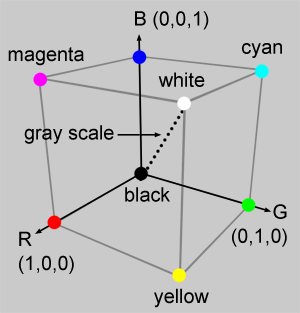
\includegraphics[width=.35\textwidth]{rgb-cube}
  % http://www.scratchapixel.com/old/lessons/3d-basic-lessons/lesson-5-colors-and-digital-images/color-spaces/
  \caption{Cubo unitário representando as cores do modelo RGB.}
  \label{fig:rgb-cube} 
\end{figure}

A origem, dada pelo vértice $(0, 0, 0)$, representa a cor preta. Já o vértice $(1, 1, 1)$, oposto à origem, representa a cor branca. Os vértices destacados sobre os eixos representam as cores primárias e os demais são o complemento de cada uma delas. Cada ponto no interior do cubo corresponde a uma cor que pode ser representada pela tripla $(r, g, b)$, onde $r, g, b \in [0, 1]$. Os tons de cinza são representados ao longo da diagonal principal do cubo, sendo que cada ponto ao longo dessa diagonal é formado por contribuições iguais de cada primária.

Vale ressaltar que existem duas formas de representar o espaço RGB: linear e não linear. O sistema supra citado mostra o modelo não linear, cuja sigla é $R'G'B'$, e é o mais utilizado por dispositivos e aplicações pela sua similaridade com o sistema visual humano. Na literatura, esse sistema é frequentemente citado com a sigla RGB, o que torna a nomenclatura dúbia, uma vez que o modelo linear também é denominado RGB e, portanto, a conversão entre os espaços de cores deve ser feita com certa cautela. Também é importante citar que os valores RGB lineares são raramente utilizados para representar uma imagem já que são, perceptualmente, altamente não uniformes \citep{konstantinos:00}.


%% ------------------------------------------------------------------------- %%
\subsection{Modelo CMY}\index{cores!modelo CMY}
\label{sec:modelo_cores_cmy}

O modelo CMY é baseado nas cores primárias complementares Ciano, Magenta e Amarelo e, diferentemente do RGB, é um modelo de cores subtrativo no qual as cores são geradas subtraindo-se o comprimento da onda dominante da luz branca e, por isso, a cor resultante corresponde à luz que é refletida \citep{gonzalez:02}.

Uma maneira de obter o sistema CMY é:\\
\begin{equation}
  \begin{bmatrix}
    C \\ M \\ Y
  \end{bmatrix} = 
  \begin{bmatrix}
    B \\ R \\ R
  \end{bmatrix} +
  \begin{bmatrix}
    G \\ B \\ G
  \end{bmatrix}
\end{equation}

ou ainda, efetuando uma mudança de coordenadas subtraindo-se as cores primárias R, G e B da cor branca $W = (1, 1, 1)$ \citep{gonzalez:02}:
\begin{equation}
  \begin{bmatrix}
    C \\ M \\ Y
  \end{bmatrix} = 
  \begin{bmatrix}
    1 \\ 1 \\ 1
  \end{bmatrix} -
  \begin{bmatrix}
    R \\ G \\ B
  \end{bmatrix}
\end{equation}

Assim como o RGB, o CMY é dependente de dispositivo. O modelo é amplamente utilizado em equipamentos que depositam pigmentos coloridos sobre papel, tais como impressoras ou fotocopiadoras coloridas.

A sobreposição das cores primárias CMY em iguais quantidades para gerar a cor preta tipicamente cria uma tonalidade próxima ao marrom ou verde escuro. Para evitar esse efeito indesejado, normalmente adiciona-se o componente de cor preta no sistema, representado pela letra $K$, obtendo-se um novo modelo conhecido como \textbf{CMYK} \citep{gonzalez:02}.

%% ------------------------------------------------------------------------- %%
\subsection{Modelo de cores da família YUV}\index{cores!modelos da família YUV}
\label{sec:modelo_cores_yuv}

O termo YUV refere-se a uma família de espaços de cores dos quais a informação de luminância, representada pelo componente Y, é codificada separadamente da crominância, dada pelos componentes U e V. Os componentes U e V são representações dos sinais da diferença do azul subtraído da luminância (B-Y) e vermelho subtraído da luminância (R-Y). É utilizado para representar as cores em sistemas de transmissão analógica de televisão nos padrões Linha de Fase Alternada (PAL) e Cor Sequencial Com Memória (SECAM) \citep{pedrini:08}.

A tranformação do espaço RGB para YUV é dada por:\\
\begin{equation}
  \begin{bmatrix}
    Y \\ U \\ V
  \end{bmatrix} = 
  \begin{bmatrix}
     0.299 &  0.587 &  0.114 \\
    -0.147 & -0.289 &  0.436 \\
     0.615 & -0.515 & -0.100 \\
  \end{bmatrix}
  \begin{bmatrix}
    R \\ G \\ B
  \end{bmatrix}
\end{equation}
onde $0 \leq R, G, B \leq 1$.

Análogo ao YUV, o modelo \textbf{YIQ} foi adotado em 1950 pelo Comitê Nacional do Sistema de Televisão (NTSC), um padrão americano para transmissão de sinal de televisão a cores. Nesse modelo, o componente Y corresponde à luminância e os componentes I (matiz) e Q (saturação) codificam a informação de crominância \citep{pedrini:08}.

A tranformação do espaço RGB para YIQ é dada por:\\
\begin{equation}
  \begin{bmatrix}
    Y \\ I \\ Q
  \end{bmatrix} = 
  \begin{bmatrix}
    0.299  &  0.587 &  0.114 \\
    0.596  & -0.275 & -0.321 \\
    0.212  & -0.523 & -0.311 \\
  \end{bmatrix}
  \begin{bmatrix}
    R \\ G \\ B
  \end{bmatrix}
\end{equation}
onde $0 \leq R, G, B \leq 1$.

Um outro modelo de cores da família YUV é o \textbf{YCbCr}, definido matematicamente por uma transformação de coordenadas em relação a algum espaço RGB \citep{pedrini:08}.

O modelo YCbCr é largamente utilizado em vídeos digitais. Nesse modelo, o componente Y representa a luminância, o componente Cb dá a medida da diferença entre a cor azul e um valor de referência, análogo ao componente Cr que é a medida da diferença entre a cor vermelha e um valor de referência \citep{pedrini:08}.

A conversão do espaço RGB para YCbCr é dada por:\\
\begin{equation}
  \begin{bmatrix}
    Y \\ Cb \\ Cr
  \end{bmatrix} = 
  \begin{bmatrix}
     0.299 &  0.587 &  0.114 \\
    -0.169 & -0.331 &  0.5   \\
     0.5   & -0.419 & -0.081 \\
  \end{bmatrix}
  \begin{bmatrix}
    R \\ G \\ B
  \end{bmatrix}
\end{equation}


%% ------------------------------------------------------------------------- %%
\subsection{Modelo de cores da família HSI}\index{cores!modelos da família HSI}
\label{sec:modelo_cores_hsi}

Modelos baseados no Matiz, Saturação e Intensidade (HSI) são mais adequados para aplicações de processamento de imagens, do ponto de vista do usuário, pela correlação com a percepção humana da cor \citep{konstantinos:00}.

Nesse modelo, assim como no YIQ, a intensidade dada pelo componente I é decomposta da informação de crominância, representada pelo matiz (H) e saturação (S) \citep{konstantinos:00}. A combinação desses componentes resulta em uma estrutura piramidal que pode ser vista na figura~\ref{fig:hsi-model}.

\begin{figure}[!h]
  \centering
  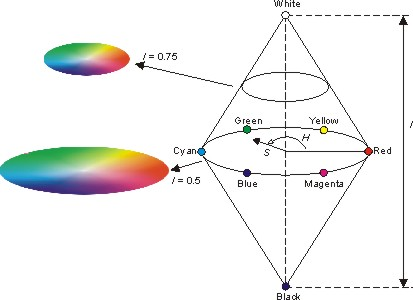
\includegraphics[width=.6\textwidth]{hsi-model}
  % http://www.blackice.com/images/HSIColorModel.jpg
  \caption{Representação gráfica do modelo HSI.}
  \label{fig:hsi-model} 
\end{figure}

O matiz descreve a cor em si, sob a forma de um ângulo $\theta$, onde $\theta \in [0, 360]$. O vermelho está situado a 0 grau, amarelo a 60, verde a 120 e assim sucessivamente. O componente de saturação, que varia entre 0 e 1, indica o quanto a cor está poluída com a cor branca. A escala de intensidade é entre $[0, 1]$, onde 0 significa preto e 1, branco.

A transformação dos componentes do espaço RGB para HSI é dada pelas equações:
\begin{align}
\label{eq:rgb_para_hsi}
\begin{split}
  \theta &= cos^{-1} \bigg( \frac{(R - G) + (R - B)}{2 \sqrt{(R - G)^2 + (R - B)(G - B)}} \bigg)
  \\
  H &= \begin{cases}
            \theta, \quad &\text{se}\ B \leq G\\
            360 - \theta, \quad &\text{caso contrário}\\
       \end{cases}
  \\
  S &= 1 - \frac{3 min(R, G, B)}{R + G + B}
  \\
  I &= \frac{R + G + B}{3}
\end{split}
\end{align}

É importante ressaltar que os valores R, G e B devem estar normalizados no intervalo entre 0 e 1. A intensidade $I$ e a saturação $S$ também estão normalizadas entre 0 e 1.

Outro modelo desta família é formado pelos componentes Matiz, Saturação e Luminância (\textbf{HSV}) e sua representação gráfica tridimensional é uma pirâmide hexagonal derivada do cubo RGB \citep{pedrini:08}.

Os vários matizes estão representados na parte superior da pirâmide, a saturação é medida ao longo do eixo horizontal e a luminância é medida ao longo do eixo vertical, que passa pelo centro da pirâmide. O matiz, que corresponde às arestas ao redor do eixo vertical, varia de 0 (vermelho) a 360 graus e o ângulo entre os vértices é de 60 graus. A saturação varia de 0 a 1 e é representada como sendo a razão entre a pureza de um determinado matiz e a sua pureza máxima, ou seja, quando $S = 1$. A luminância varia de 0, no pico da pirâmide representando a cor preta, a 1 na base, onde as intensidades das cores são máximas \citep{pedrini:08}.

A conversão do espaço RGB para HSV é dada pelas equações:
\begin{align}
\label{eq:rgb_para_hsv}
\begin{split}
  H &=  \begin{cases}
            60\frac{(G - B)}{M - m}, \quad &\text{se}\ M = R\\
            60\frac{(B - R)}{M - m} + 120, \quad &\text{se}\ M = G\\
            60\frac{(R - G)}{M - m} + 240, \quad &\text{se}\ M = B\\
       \end{cases}
  \\
  S &=  \begin{cases}
            \frac{(M - m)}{M}, \quad &\text{se}\ M \neq 0\\
            0, \quad &\text{caso contrário}\\
       \end{cases}
  \\
  V &= M
\end{split}
\end{align}

\noindent onde $m = min(R, G ,B)$ e $M = max(R, G ,B)$. A luminância $V$ e a saturação $S$ estão normalizadas entre 0 e 1. Já o matiz $H$ varia entre 0 e 360 graus.

Da mesma forma que o HSV, o modelo Matiz, Saturação e Luminosidade (\textbf{HSL}) é uma representação tridimensional e é formado por dois cones de altura 1, cujas bases são coincidentes \citep{pedrini:08}.

O matiz é determinado pelos pontos no círculo das bases comuns aos cones. A saturação varia de 0 a 1, conforme a distância ao eixo do cone. A luminosidade está ao longo do eixo vertical comum aos dois cones e varia na escala $[0, 1]$, onde 0 significa preto e 1, branco \citep{pedrini:08}.

A conversão do espaço RGB para HSL é dada pelas equações:
\begin{align}
\label{eq:rgb_para_hsl}
\begin{split}
  H &=  \begin{cases}
            60\frac{(G - B)}{M - m}, \quad &\text{se}\ M = R\\
            60\frac{(B - R)}{M - m} + 120, \quad &\text{se}\ M = G\\
            60\frac{(R - G)}{M - m} + 240, \quad &\text{se}\ M = B\\
       \end{cases}
  \\
  S &=  \begin{cases}
            \frac{(M - m)}{M + m}, \quad &\text{se}\ 0 < L \leq 0,5\\
            \frac{(M - m)}{2 - (M + m)}, \quad &\text{se}\ L > 0,5\\
            0, \quad &\text{se}\ M = m\\
       \end{cases}
  \\
  L &= \frac{M + m}{2}
\end{split}
\end{align}

\noindent onde $m = min(R, G ,B)$ e $M = max(R, G ,B)$. A luminância $V$ e a saturação $S$ estão normalizadas entre 0 e 1. Observe que a transformação do matiz $H$ é a mesma utilizada na conversão do espaço RGB para HSV em \ref{eq:rgb_para_hsv} e varia entre 0 e 360 graus.

Todos os modelos de cores desta família têm a propriedade de se pensar em cores mais claras, obtidas pelo aumento do brilho ou luminosidade, e mais escuras, pela diminuição dos mesmos valores. As cores intermediárias são produzidas pela diminuição da saturação \citep{pedrini:08}.

%% ------------------------------------------------------------------------- %%
\section{Teoria \emph{fuzzy}}\index{fuzzy!teoria}
\label{sec:teoria_fuzzy}

Em muitos problemas, não há dificuldade em determinar se um dado elemento é ou não parte de um grupo. Essa ideia vem da teoria clássica de conjuntos e é embasada no conceito fundamental de conjunto \citep{chen:00}. Pode-se, por exemplo, afirmar que o número $7$ pertence ao conjunto dos números naturais e, da mesma maneira, que o número $-7$ não pertence a esse mesmo conjunto. Este é um caso clássico em que a aplicação da lógica booleana é bem sucedida. Em outras palavras, quando questionado se o número $7$ pertence ao conjunto dos naturais tem-se, apenas, duas respostas possíveis: sim ou não.

Entretanto, há inúmeros indivíduos ou observações na natureza que nem sempre podem ser classificados de tal forma, pelo fato de que a relação de pertinência não é bem definida \citep{pedrycz:98}. Como exemplo, o conjunto das pessoas altas, os números reais aproximadamente zero ou o grupo de alunos mais inteligentes da escola. Ocorre que, nesses casos, a aplicação da lógica booleana para classificar elementos como parte de um grupo ou não é imprecisa. Em outras palavras, se tomado $x = 1,70m$ como o limiar que separa as pessoas altas das baixas, fica evidente que a utilização da lógica booleana não resulta em interpretações realísticas, pois uma pessoa com $1,69m$ é, portanto, baixa ou, pode-se dizer ainda, que não pertence ao grupo das pessoas altas. Ora, apenas $1$ centímetro separa tal pessoa de um grupo ou de outro. Analogamente, uma pessoa com $1,71m$ está muito próxima de pertencer ao grupo das pessoas baixas.

Claramente, a resposta a ser obtida quando da análise de possibilidades desse tipo é fortemente dependente do contexto, pois há um alto grau de incerteza inerente aos elementos e conjuntos sendo considerados.

O conceito de incerteza mudou gradativamente na ciência e na matemática. Na ciência, esta mudança foi manifestada por uma transição gradual da visão tradicional, que insiste que a incerteza é indesejável e, por esta razão, ela deve ser evitada por todos os meios possíveis, para uma visão alternativa, que é tolerante à incerteza. De acordo com a visão tradicional, a ciência deve esforçar-se de certeza em todas as suas manifestações, ou seja, com precisão, especificidade, nitidez, consistência e, por conseguinte, a incerteza é considerada como não científica. De acordo com a visão alternativa, a dúvida é considerada essencial para a ciência; não é só uma praga inevitável, mas tem, de fato, uma grande utilidade \citep{klir:95}.

E com base na ideia moderna de que a incerteza é algo útil na ciência é que Zadeh convergiu para um de seus mais importantes trabalhos: a teoria de conjuntos \emph{fuzzy}, cuja abordagem sobre conjuntos dá-se sob a ótica de que os limites entre eles não são precisos e, portanto, é possível estabelecer funções que forneçam um certo \textbf{grau de pertinência} de um elemento a um dado conjunto \citep{zadeh:65}.

A capacidade de conjuntos \emph{fuzzy} expressarem transições graduais de pertinência e não pertinência tem uma grande utilidade. Ela fornece não só uma representação significativa e poderosa da medida de incerteza, mas também uma forma de expressar conceitos vagos em linguagem natural \citep{klir:95}. Voltando ao exemplo do conjunto de pessoas altas, em vez de descrever a altura de uma pessoa com exatidão em metros ou centímetros, pode-se apenas dizer que ela é alta, baixa ou mediana. Cada um desses conjuntos pode ser um conjunto \emph{fuzzy}, onde um valor 1 é atribuído a um membro que está totalmente incluído em um deles, ou 0 caso contrário. Valores intermediários nessa escala indicam que o elemento está parcialmente em um dos conjuntos.

A seção \ref{sec:conjuntos_fuzzy} explicita algumas das definições formais e conceitos básicos da teoria dos conjuntos \emph{fuzzy} proposta por Zadeh.

%% ------------------------------------------------------------------------- %%
\subsection{Conjuntos \emph{fuzzy}}\index{fuzzy!conjuntos}
\label{sec:conjuntos_fuzzy}
A teoria de conjuntos clássicos está baseada em uma função, geralmente conhecida como função característica, dada por:

\begin{equation}
  \mu_A(x) =  \begin{cases}
                1 \quad \text{se}\ x \in A \\
                0 \quad \text{se}\ x \notin A
              \end{cases}
\end{equation}
onde $U$ é o conjunto Universo, $A$ é um subconjunto de $U$ e $x$ é um elemento de $U$ \citep{klir:95}.

Portanto, a função característica é um mapeamento dos elementos de $U$ no conjunto binário $\{0, 1\}$, formalmente definida como:

\begin{equation}
  \mu_A =  U \rightarrow \{0, 1\}
\end{equation}

Sendo assim, a função característica determina que, de acordo com algum critério, $\forall x \in U$, se $\mu_A(x) = 1$, então $x$ é um membro de $A$, por outro lado, quando $\mu_A(x) = 0$, $x$ não é um membro de $A$.

Quanto aos conjuntos \emph{fuzzy}, basta generalizar a função característica aplicada nos conjuntos clássicos no intervalo $[0, 1]$ para obter-se um conjunto "fuzzificado", ou seja, o grau de pertinência de um elemento $x$ passa, agora, a ser expresso em termos contínuos. Em outras palavras, o elemento $x$ pertence ao subconjunto $A$ de $U$ com algum grau de pertinência obtido do intervalo $[0, 1]$. Formalmente, tem-se:

\begin{equation}
  \mu_A =  U \rightarrow [0, 1]
\end{equation}

Cabe aqui citar a definição de conjuntos \emph{fuzzy} dada por Zadeh que designa um conjunto \emph{fuzzy} como uma classe de objetos com um grau de pertinência contínuo. Tal conjunto é caracterizado por uma função de pertinência (característica), que atribui a cada objeto um grau de pertinência que varia entre zero e um. As noções de inclusão, união, intersecção, complemento, relação, convexidade, etc., oriundas da teoria de conjuntos clássica, são estendidas a esses conjuntos \citep{zadeh:65}.

% definição de conjunto fuzzy
\begin{defn}
Um conjunto \emph{fuzzy} $A$ é um subconjunto do conjunto universo $U$ formado por pares ordenados de um elemento qualquer $x$ e seu grau de pertinência dado por $\mu_A(x)$, da forma:

\begin{equation}
  A =  \{(x, \mu_A(x)) \ |\ x \in U\}
\end{equation}
\end{defn}

O universo de discurso $U$ pode ser composto por elementos discretos ou ser um espaço contínuo. A mesma implicação vale para o subconjunto $A$. No caso em que $U$ é um conjunto discreto e finito, tal que $U = \{x_1, x_2, x_3, \ldots, x_n\}$, pode-se simplesmente enumerar os seus elementos, juntamente com seus graus de pertinência, como segue:

\begin{equation}
  A =  \frac{\mu_A(x_1)}{x_1} + \frac{\mu_A(x_2)}{x_2} + \ldots + \frac{\mu_A(x_n)}{x_n} = \sum_{i=1}^n \frac{\mu_A(x_i)}{x_i}
\label{equ:conjunto_fuzzy_finito}
\end{equation}

É importante ressaltar que o somatório em \ref{equ:conjunto_fuzzy_finito} não significa uma adição algébrica, mas sim a união de todos os pares ordenados de $x$ e $\mu_A(x)$ que formam o conjunto $A$ \citep{klir:95}.

\begin{exmp}
\textcolor{red}{Colocar um exemplo aqui de conjunto fuzzy que tenha sentido com o restante do texto, posteriormente. Pode ser pessoas altas, para ligar com o exemplo supra citado.}
\end{exmp}

% definição de altura
\begin{defn}
A altura de $A$, denotado por $altura(A)$, corresponde ao limite superior do codomínio da sua função de pertinência, da forma:

\begin{equation}
  altura(A) = \{\mu_A(x) \ |\ x \in U\}
\label{equ:conjunto_fuzzy_altura}
\end{equation}

\end{defn}

% definição de conjunto normalizado
\begin{defn}
Um conjunto \emph{fuzzy} $A$ é dito normalizado se existe pelo menos um elemento $x \in U$, tal que $\mu_A(x) = 1$.
\label{def:conjunto_fuzzy_normalizado}
\end{defn}

A definição de conjunto \emph{fuzzy} normalizado implica que pelo menos um membro de $A$ alcança o grau de pertinência máximo possível. Note que a definição em \ref{def:conjunto_fuzzy_normalizado} considera que os valores dos graus de pertinência variam no intervalo fechado entre 0 e 1. Logo, no mínimo um elemento deve ter um grau de pertinência 1 para que $A$ possa ser considerado, de fato, normalizado. Observe que, decorrente dessa afirmação, imediatamente tem-se que que $altura(A) = 1$.

% definição de suporte
\begin{defn}
O suporte de um conjunto \emph{fuzzy} $A$ em $U$, denotado por $suporte(A)$, é o conjunto dado por:

\begin{equation}
  suporte(A) = \{x \in U \ |\ \mu_A(x) > 0 \}
\label{equ:conjunto_fuzzy_suporte}
\end{equation}

\end{defn}

Em outras palavras, o conjunto suporte é um conjunto clássico ou conjunto ordinário que contém todos os elementos de $U$ cujo grau de pertinência é maior do que zero em $A$. Denomina-se por conjunto unitário ou \emph{singleton} um conjunto \emph{fuzzy} cujo suporte é um único ponto, por exemplo $w$, tal que $\mu_A(w) = 1$.

% definição de alfa corte
\begin{defn}
Um $\alpha$\emph{-corte}, também conhecido por $\alpha$\emph{-nível}, é o subconjunto clássico de elementos cujo grau de pertinência é maior ou igual a um valor $\alpha$, formalmente:

\begin{equation}
  \alpha\emph{-corte(A)} = \{x \in U \ |\ \mu_A(x) \geq \alpha \}
\label{equ:conjunto_fuzzy_alpha_corte}
\end{equation}
\end{defn}

% definição de núcleo
\begin{defn}
O núcleo ou \emph{kernel} de um conjunto \emph{fuzzy} $A$ em $U$, é o conjunto de elementos pertencentes inteiramente à $A$, da forma:

\begin{equation}
  \emph{núcleo}(A) = \{x \in U \ |\ \mu_A(x) = 1 \}
\label{equ:conjunto_fuzzy_kernel}
\end{equation}
\end{defn}

Vale destacar que, por construção, o núcleo do conjunto $A$ está contido no conjunto suporte, o que pode ser representado formalmente como $\emph{núcleo}(A) \subseteq suporte(A)$.

A figura~\ref{fig:fuzzy_definitions} mostra graficamente algumas das propriedades definidas acima.

\begin{figure}[!h]
  \centering
  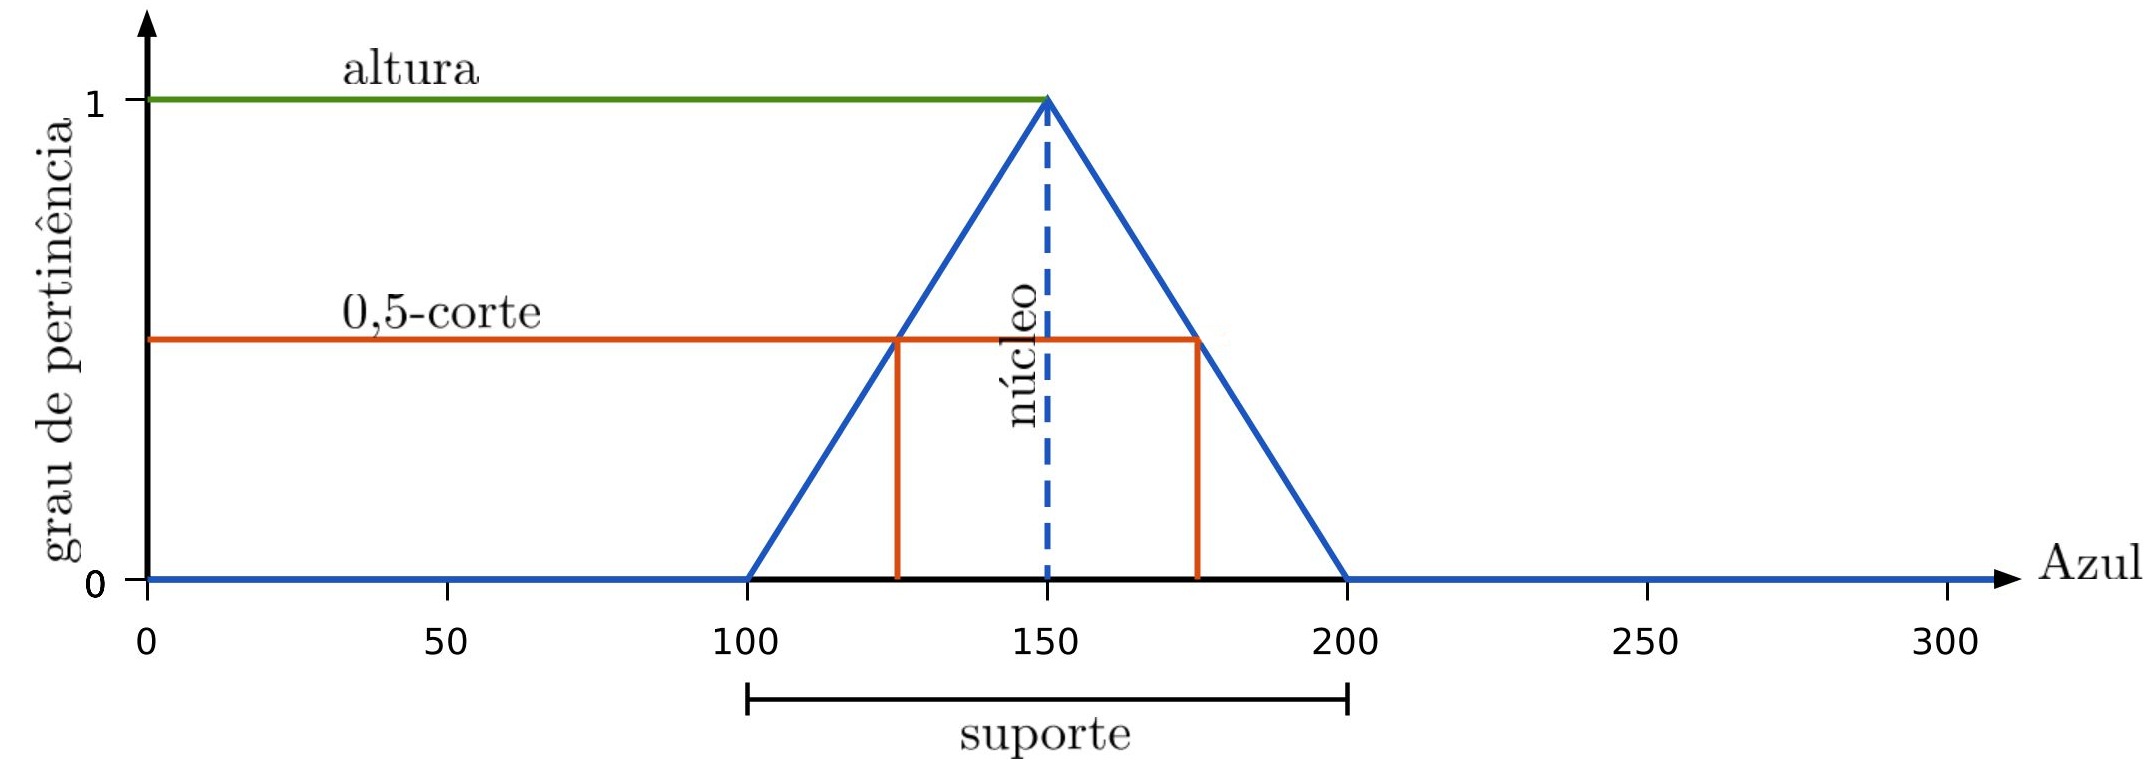
\includegraphics[width=1\textwidth]{fuzzy_definitions}
  % source MIT class notes
  \caption{Representação gráfica das principais propriedades dos conjuntos fuzzy. Detalhar melhor e corrigir a imagem.}
  \label{fig:fuzzy_definitions} 
\end{figure}

%% ------------------------------------------------------------------------- %%
\subsection{Operações entre conjuntos \emph{fuzzy}}\index{fuzzy!operações entre conjuntos}

Assim como na teoria de conjuntos clássica, há basicamente três operações que podem ser estendidas aos conjuntos \emph{fuzzy}. Essas operações são a união, a intersecção e o complemento, sendo representadas pelos operadores lógicos de conjunção (\textbf{OU}), disjunção (\textbf{E}) e complemento \textbf{NÃO}, respectivamente. As operações básicas formam o que é conhecido como \textbf{operações padrão em conjuntos \emph{fuzzy}} \citep{klir:95}.

Tais operações são realizadas sobre suas respectivas funções de pertinência e há muitas formalizações matemáticas possíveis para os operadores que representam-nas. O par de operadores mais amplamente utilizado é o operador de mínimo ($min$) e máximo ($max$), que são semelhantes aos operadores produto e soma da álgebra elementar e utilizados para expressar a conjunção e disjunção, respectivamente \citep{thole:79}.

Seja dois conjuntos \emph{fuzzy} $A$ e $B$, definidos sobre um mesmo universo de discurso $U$. Utilizando as funções $max$ e $min$, tem-se que \citep{klir:95}:

% definição de união
\begin{defn}
\label{def:conjunto_fuzzy_uniao}
O conjunto união é formado por todos os valores máximos entre dois conjuntos \emph{fuzzy} $A$ e $B$, onde $A, B \in U$, da forma:

\begin{equation}
  \mu_A(x) \cup \mu_B(x) = max\{\mu_A(x), \mu_B(x)\}, \quad \forall x \in U
\end{equation}
\end{defn}

% definição de intersecção
\begin{defn}
\label{def:conjunto_fuzzy_interseccao}
O conjunto intersecção é formado por todos os valores mínimos entre dois conjuntos \emph{fuzzy} $A$ e $B$, onde $A, B \in U$, da forma:

\begin{equation}
  \mu_A(x) \cap \mu_B(x) = min\{\mu_A(x), \mu_B(x)\}, \quad \forall x \in U
\end{equation}
\end{defn}

% definição de complemento
\begin{defn}
\label{equ:conjunto_fuzzy_complemento}
O complemento de um conjunto \emph{fuzzy} $A$, denotado por $\mu_{\bar{A}}(x)$, onde $A \in U$, é formado pela subtração entre o valor unitário e $\mu_A(x)$, da forma:

\begin{equation}
  \mu_{\bar{A}}(x) = 1 - \mu_A(x), \quad \forall x \in U
\end{equation}
\end{defn}

Além desses operadores, existem outros que podem ser utilizados para efetuar as operações lógicas. Um deles é a norma triangular, também denominada \textbf{\emph{norma-t}}, e co-norma triangular, usualmente denominada por \textbf{\emph{co-norma-t}} ou \textbf{\emph{norma-s}}. Os operadores utilizados para a intersecção de conjuntos \emph{fuzzy} pertencem à classe \emph{norma-t}. Os operadores utilizados para a união de conjuntos \emph{fuzzy} pertencem à classe \emph{co-norma-t} ou \emph{norma-s} \citep{zimmermann:01}.

Ambas \emph{norma-t} e \emph{norma-s} são funções binárias do tipo $[0, 1] \times [0, 1] \rightarrow [0, 1]$, que devem satisfazer algumas propriedades, tais como, monotonicidade, comutatividade, associatividade e condições de contorno \footnote{As propriedades não serão expressas neste trabalho, embora sejam amplamente conhecidas, exceto pelas condições de contorno. Mais detalhes podem ser vistos em \citet{zimmermann:01}.}. Os operadores $max$ e $min$ satisfazem tais propriedades e, por essa razão, podem ser utilizados nas operações lógicas \emph{fuzzy} \citep{zimmermann:01}.


%% ------------------------------------------------------------------------- %%
\subsection{Números \emph{fuzzy}}
\label{sec:numeros_fuzzy}
Texto texto texto texto texto texto texto texto texto texto texto texto texto
texto texto texto texto texto texto texto.


%% ------------------------------------------------------------------------- %%
\subsection{Funções de pertinência}
\label{sec:funcoes_pertinencia}
Texto texto texto texto texto texto texto texto texto texto texto texto texto
texto texto texto texto texto texto texto.


%% ------------------------------------------------------------------------- %%
\subsection{Variáveis linguísticas}
\label{sec:variaveis_linguisticas}
Texto texto texto texto texto texto texto texto texto texto texto texto texto
texto texto texto texto texto texto texto.


%% ------------------------------------------------------------------------- %%
\subsection{Sistemas baseados em regras \emph{fuzzy}}\index{fuzzy!sistemas baseados em regras}
\label{sec:sistemas_regras_fuzzy}
Texto texto texto texto texto texto texto texto texto texto texto texto texto
texto texto texto texto texto texto texto.










%% ------------------------------------------------------------------------- %%
\begin{comment}
\section{Exemplo de Código-Fonte em Java}
\label{sec:exemplo_codigo_fonte}
Texto texto texto texto texto texto texto texto texto texto texto texto texto
texto texto texto texto texto texto texto texto texto texto texto texto texto
texto texto texto texto texto texto texto texto texto texto texto texto texto
texto texto texto texto texto texto texto.

% Foi utilizado o pacote listing para formatar código fonte
% http://ctan.org/tex-archive/macros/latex/contrib/listings/listings.pdf
% Veja no preambulo do arquivo tese-exemplo.tex os parâmetros de configuração.

\begin{lstlisting}[frame=trbl]
   for(i = 0; i < 20; i++)
   {
       // Comentário 
       System.out.println("Mensagem...");
   }
\end{lstlisting}


%% ------------------------------------------------------------------------- %%
\section{Algumas Referências}
\label{sec:algumas_referencias}

É muito recomendável a utilização de arquivos \emph{bibtex} para o gerenciamento
de referências a trabalhos. Nesse sentido existem três plataformas gratuitas
que permitem a busca de referências acadêmicas em formato bib: 
\begin{itemize}
	\item \emph{CiteULike} (patrocinados por Springer): \url{www.citeulike.org}
	\item Coleção de bibliografia em Ciência da Computação: \url{liinwww.ira.uka.de/bibliography}
	\item Google acadêmico (habilitar bibtex nas preferências): \url{scholar.google.com.br}
\end{itemize}
Lamentavelmente, ainda não existe um mecanismo de verificação ou validação das
informações nessas plataformas. Portanto, é fortemente sugerido validar todas
as informações de tal forma que as entradas bib estejam corretas.  Também, tome
muito cuidado na padronização das referências bibliográficas: ou considere TODOS
os nomes dos autores por extenso, ou TODOS os nomes dos autores abreviados.
Evite misturas inapropriadas.

Exemplos de referências com a tag:
\begin{itemize}

\item @InCollection: \citep{bobaoglu93:concepts}.
{\scriptsize\begin{verbatim}
@InCollection{bobaoglu93:concepts,
 author   = {Ozalp Babaoglu and Keith Marzullo},
 title    = {Consistent Global States of Distributed Systems: Fundamental Concepts
            and Mechanisms},
 editor   = {Sape Mullender},
 booktitle= {Distributed Systems},
 edition  = {segunda},
 year     = {1993},
 pages    = {55-96}
}
\end{verbatim}}

\item @Conference: \citep{bronevetsky02}.
{\scriptsize\begin{verbatim}
@Conference{bronevetsky02,
 author   = {Greg Bronevetsky and Daniel Marques and Keshav Pingali and 
            Paul Stodghill},
 title    = {Automated application-level checkpointing of {MPI} programs},
 booktitle= {PPoPP '03: Proceedings of the 9th ACM SIGPLAN Symposium on Principles
            and Practice of Parallel Programming},
 year     = {2003},
 pages    = {84-89}
}
\end{verbatim}}

\item @PhdThesis: \citep{garcia01:PhD}.
{\scriptsize\begin{verbatim}
@PhdThesis{garcia01:PhD,
 author   = {Islene C. Garcia},
 title    = {Visões Progressivas de Computações Distribuídas},
 school   = {Instituto de Computação, Universidade de Campinas, Brasil},
 year     = {2001},
 month    = {Dezembro}
}
\end{verbatim}}

\item @MastersThesis: \citep{schmidt03:MSc}.
{\scriptsize\begin{verbatim}
@MastersThesis{schmidt03:MSc,
 author   = {Rodrigo M. Schmidt},
 title    = {Coleta de Lixo para Protocolos de \emph{Checkpointing}},
 school   = {Instituto de Computação, Universidade de Campinas, Brasil},
 year     = {2003},
 month    = Oct
}
\end{verbatim}}

\item @Techreport: \citep{alvisi99:analysisCIC}.
{\scriptsize\begin{verbatim}
@Techreport{alvisi99:analysisCIC,
 author   = {Lorenzo Alvisi and Elmootazbellah Elnozahy and Sriram S. Rao and
            Syed A. Husain and Asanka Del Mel},
 title    = {An Analysis of Comunication-Induced Checkpointing},
 institution= {Department of Computer Science, University of Texas at Austin},
 year     = {1999},
 number   = {TR-99-01},
 address  = {Austin, {USA}}
}
\end{verbatim}}

\item @Manual: \citep{CORBA:spec}.
{\scriptsize\begin{verbatim}
@Manual{CORBA:spec,
 title    = {{CORBA v3.0 Specification}},
 author   = {{Object Management Group}},
 month    = Jul,
 year     = {2002},
 note     = {{OMG Document 02-06-33}}
}
\end{verbatim}}

\item @Misc: \citep{gridftp}.
{\scriptsize\begin{verbatim}
@Misc{gridftp,
 author   = {William Allcock},
 title    = {{GridFTP} protocol specification. {Global Grid Forum}
            Recommendation ({GFD}.20)},
 year     = {2003}
}
\end{verbatim}}

\item @Misc: para referência a artigo online \citep{fowler04:designDead}.
{\scriptsize\begin{verbatim}
@Misc{fowler04:designDead,
 author   = {Martin Fowler},
 title    = {Is Design Dead?},
 year     = {2004},
 month    = May,
 note     = {Último acesso em 30/1/2010},
 howpublished= {\url{http://martinfowler.com/articles/designDead.html}},
}
\end{verbatim}}

\item @Misc: para referência a página web \citep{FSF:GNU-GPL}.
{\scriptsize\begin{verbatim}
@Misc{FSF:GNU-GPL,
 author   = {Free Software Foundation},
 title    = {GNU general public license},
 year     = {2007},
 note     = {Último acesso em 30/1/2010},
 howpublished= {\url{http://www.gnu.org/copyleft/gpl.html}},
}
\end{verbatim}}

\end{itemize}
\end{comment}
